\documentclass[a4paper,10pt]{report}
\usepackage[french]{babel}
\usepackage[utf8]{inputenc}
\usepackage[left=2.5cm,top=2cm,right=2.5cm,nohead,nofoot]{geometry}
\usepackage{url}
\usepackage{graphicx}

\linespread{1.1}



\begin{document}

\begin{titlepage}
\begin{center}
\textbf{\textsc{UNIVERSIT\'E LIBRE DE BRUXELLES}}\\
%\textbf{\textsc{Faculté des Sciences}}\\
%\textbf{\textsc{Département d'Informatique}}
\vfill{}\vfill{}
\begin{center}{\Huge Rapport : Villo !}\end{center}{\Huge \par}
\begin{center}{\large Pierre Gérard, Titouan Christophe}\end{center}{\Huge \par}
\vfill{}\vfill{} \vfill{}
\begin{flushleft}{\large \textbf{INFO-H-303 Base de données}}\hfill{Esteban Zimányi, Michaël Waumans}\end{flushleft}{\large\par}
\vfill{}\vfill{}\enlargethispage{3cm}
\textbf{Année académique 2014~-~2015}
\end{center}
\end{titlepage}

%\begin{abstract}
%Ce rapport présente ...
%\end{abstract}


\tableofcontents


\chapter{Diagramme entité association}
\section{Diagramme}
\begin{figure}[hbt]
  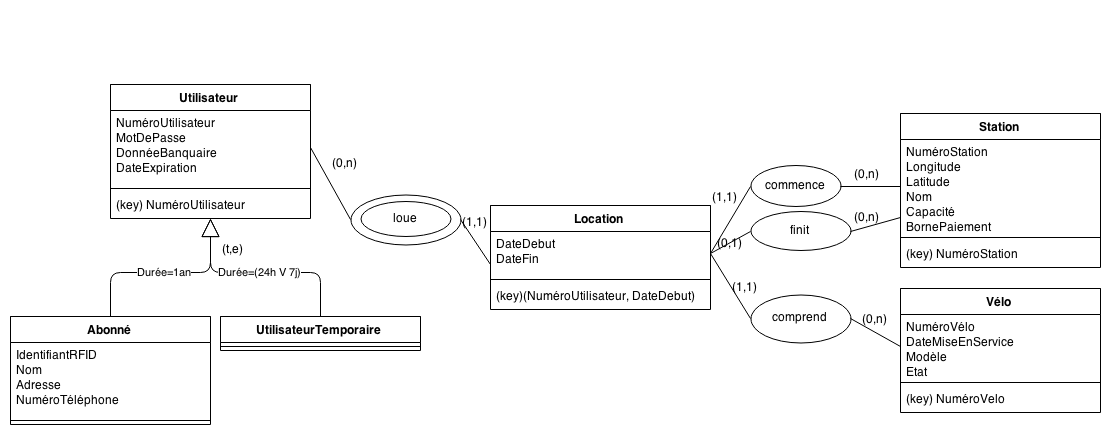
\includegraphics[scale=0.4]{dia/diagramme-entite-association.png}
  \caption{Diagramme entité association
}
\end{figure}
\section{Contraintes}
Les contraintes sont les suivantes :
\begin{itemize}
  \item La DateDebut d'une Location doit précéder la DateFin, 
  \item La DateMiseEnService d'un Vélo doit précéder la DateDebut de chacune de ses Locations,
  \item La DateExpiration d'un Utilisateur doit précéder la DateDebut de toutes ses Locations,
  \item La DateExpiration d'un Utilisateur doit \^etre postérieur à la DateFin de toutes ses Locations,
  \item Les intervalles entre DateDébut et DateFin de deux Location pour un même Vélo ou un même Utilisateur ne peuvent pas se chevaucher,
  \item Pour une Station, le nombre de vélo dont la dernière Location finit  dans cette station ne doit pas dépasser sa capacité,
  \item Un Vélo ne peut pas avoir de déplacement disjoints.
  \item Un Utilisateur ayant une DateExpiration ne peut pas prendre un Vélo si Usable est faux.
\end{itemize}
\section{Hypothèses et justifications}

% que ce passe-t-il si un utilisateur est temporaire puis s'abonne?

Il existe des utilisateur "admin", c'est ces derniers et uniquement eux qui n'ont pas de date d'expiration.

Si un Abonné a son abonnement qui expire, il peut re-utiliser le NuméroUtilisateur et MotDePasse dans le futur, l'entité n'est pas supprimé. Pour UtilisateurTemporaire, l'entité peut être supprimé.

Dans le cas ou des employés villo déplace un vélo la nuit, alors ce déplacement doit être enregistré dans la base de donnée par un utilisateur admin.

Dans le cas ou un vélo serait cassé et devrait sortir du circuit de location, un Utilisateur admin vient le chercher et la Location ne finit jamais, c'est à dire pas de DateFin.

Dans le cas ou la société villo achète des nouveaux vélo et les mets en circulation, un utilisateur admin fait une location de ce nouveau vélo qui a une date de départ égale à la date d'arrivée et une station de départ égale à la station d'arrivée.

Le champs MotDePasse contient un hash cryptographique du mot de passe et non le mot de passe lui-m\^eme.


\chapter{Modèle relationnel}
\section{Modèle}

% ca cté du bo latek une fois
\begin{description}
\item[] \textbf{Utilisateur}(\underline{NuméroUtilisateur}, MotDePasse, DonnéeBanquaire, \textit{DateExpiration})

\item[] \textbf{Abonné}(IdentifiantRFID, Nom, Adresse, NuméroTélephone)
	% ICI herirtage ? Une des trois solution proposé

\item[] \textbf{UtilisateurTemporaire}()
	%ICI heritage ?

\item[] \textbf{Location}(\underline{NuméroUtilisateur,DateDebut},\textit{DateFin}, NuméroStationDépart , NuméroStationFin, NuméroVélo) % par sur de la notation pour NuméroStationDépart ???
	\begin{description}
	\item[] NuméroUtilisateur référence Utilisateur.NuméroUtilisateur
	\item[] NuméroVélo référence Vélo.NuméroVélo
	\item[] NuméroStationDépart référence Station.NuméroStation
	\item[] NuméroStationFin référence Station.NuméroStation
	\end{description}
	
\item[] \textbf{Station}(\underline{NuméroStation}, Longitude, Latitude, Nom, Capacité, BornePaiement)

 \item[] \textbf{Vélo}(\underline{NuméroVélo}, DateMiseEnService, Modèle, Etat)

\end{description}

\section{Contraintes}
\section{Hypothèses et justifications}




\end{document}